\section{Rails Web Servers} % (fold)
\label{tech:sec:rails_webservers}
In its simplest manner, a web server is a never ending \textit{loop} that accepts connections on a listening \textit{socket} and handles them somehow. There are notorious differences on how this \textit{loop} is implemented, besides the classical architectural and philosophical differences behind each web server. These differ in handling multi processing, multi threading, asynchronous events, data copying, context switching, locking contention, memory management, blocking operations, HTTP parsing, the TCP stack implementation and many other architectural differences.


\subsection{WEBrick}
This is Ruby's pioneer web server. It was created in 2000 by Masayoshi Takahashi and Yuuzou Gotou. WEBrick is a full-featured server that supports HTTP, HTTPS and listening concurrently to several ports, among other features. It is purely written in Ruby and has a very modular design, allowing developers to extend its functionalities by supporting external handlers~\cite{webrick_guide}.
WEBrick uses a single process but spawns a new thread for each incoming request. Mainly due to being written in Ruby, its HTTP parser is known for its poor performance~\cite{ruby_webservers}. WEBrick's request handling is demonstrated on figure~\ref{fig:webrick_architecture}.
\begin{figure}[h!t]
  \centering
  \caption{WEBrick's Request Handling Process}
  \label{fig:webrick_architecture}
    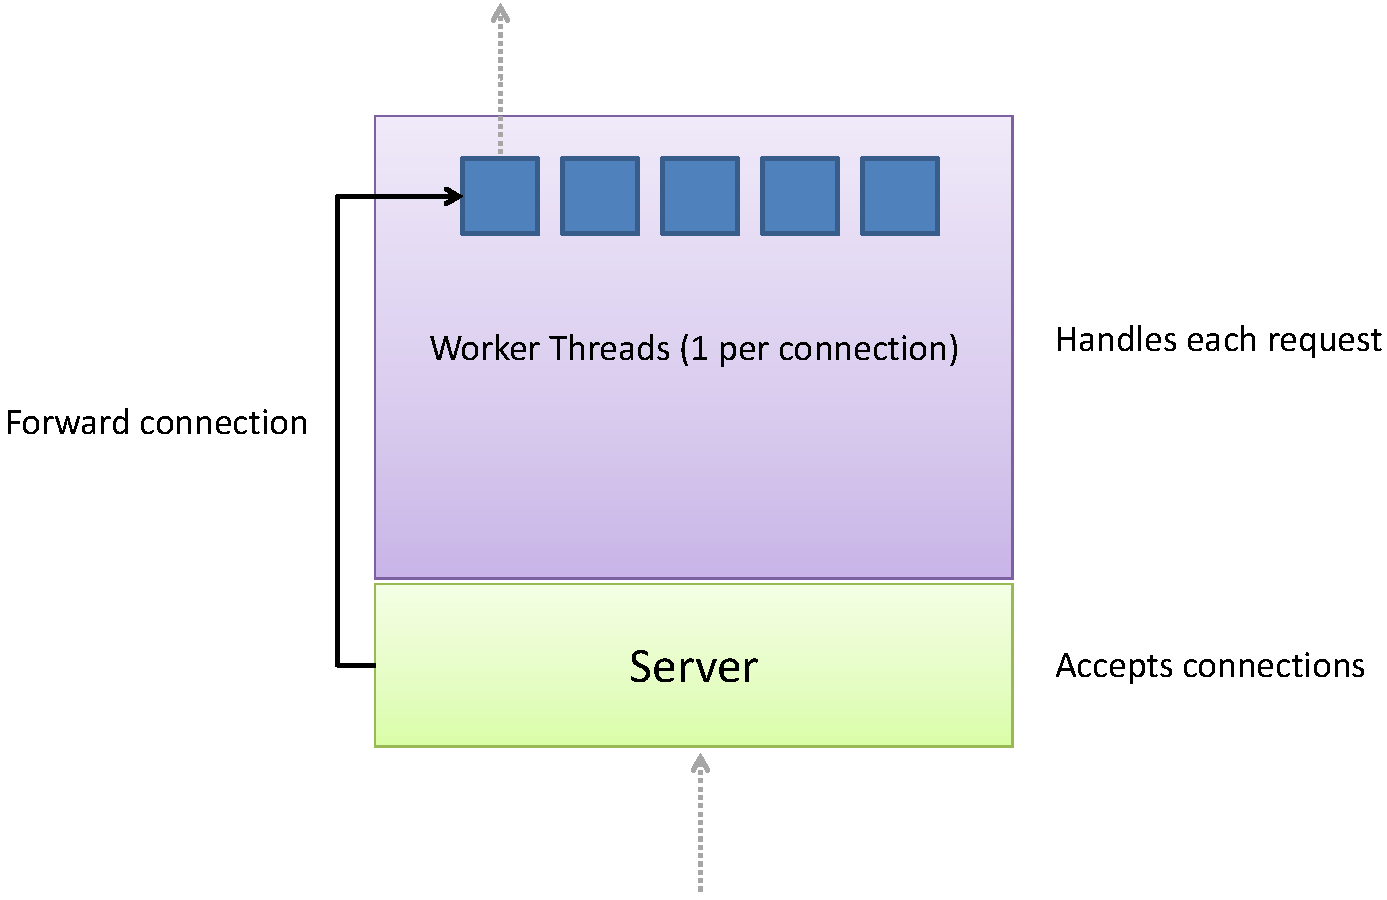
\includegraphics[width=0.75\textwidth]{webrick_architecture}
\end{figure}
Due to its poor performance, users normally used alternate, less conventional setups which were also known for their poor stability~\cite{ruby_webservers}.


\subsection{Mongrel}
Mongrel was released by Zed A. Shaw in 2006 and soon became the most popular web server used to run Rails applications. It offered a much better performance when compared to WEBrick and it was reasonably suited for production environments. This was mainly due to its improved implementation of the HTTP parser, which was rewritten in C~\cite{mongrel_server_production}.

Similarly to WEBrick, Mongrel uses a single process. It has an acceptor thread which handles every incoming connections, launching new threads for each one of them. In production environments, Mongrel is commonly found in clustered configurations where several processes are launched and their usage is dictated by a proxy server~\cite{mongrel_faq}. Mongrel's request handling is demonstrated on figure~\ref{fig:mongrel_architecture}.
\begin{figure}[h!t]
  \centering
  \caption{Mongrel's Request Handling Process}
  \label{fig:mongrel_architecture}
    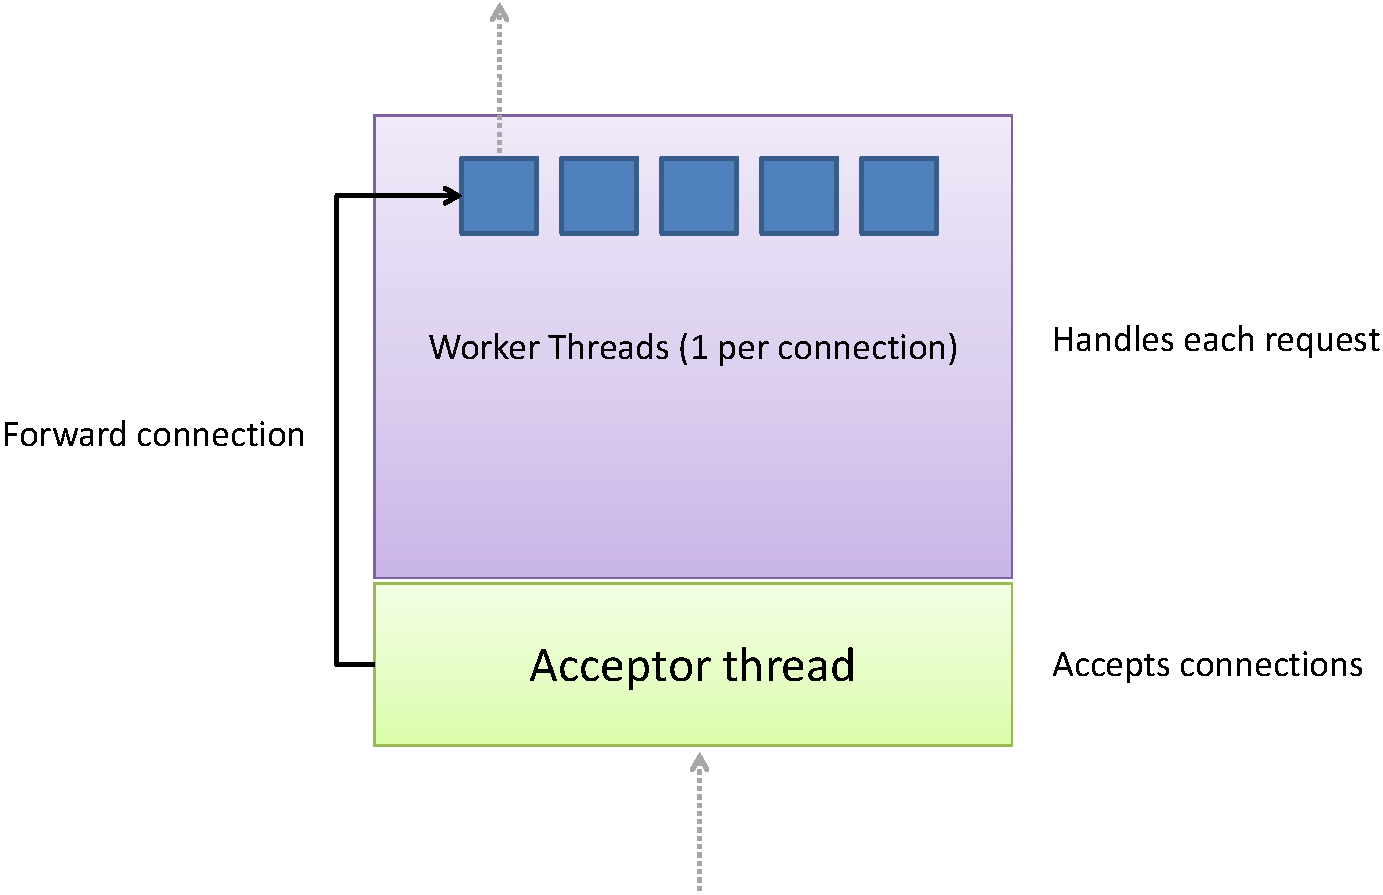
\includegraphics[width=0.75\textwidth]{mongrel_architecture}
\end{figure}
Mongrel also optimized the TCP stack by changing Ruby's default socket listening queue from 5 to 1024, besides using optimization flags on socket connections to improve bandwidth usage~\cite{mongrel_faq}.


\subsection{Thin}
Thin was released in 2008 and was the first Ruby web server which did not follow the \textit{one thread per request} convention. It uses Mongrel's HTTP parser and EventMachine as its I/O back-end, allowing it to use a fast asynchronous event loop in a single thread for all incoming requests~\cite{thin}. Thin recently became able to combine threading with its philosophy, by allowing the creation of a background pool of 20 threads~\cite{ruby_webservers}. Thin is written in C, C++ and Ruby and is optimized for small requests and fast clients. Its request handling is demonstrated on figure~\ref{fig:thin_architecture}.
\begin{figure}[h!t]
  \centering
  \caption{Thin's Request Handling Process}
  \label{fig:thin_architecture}
    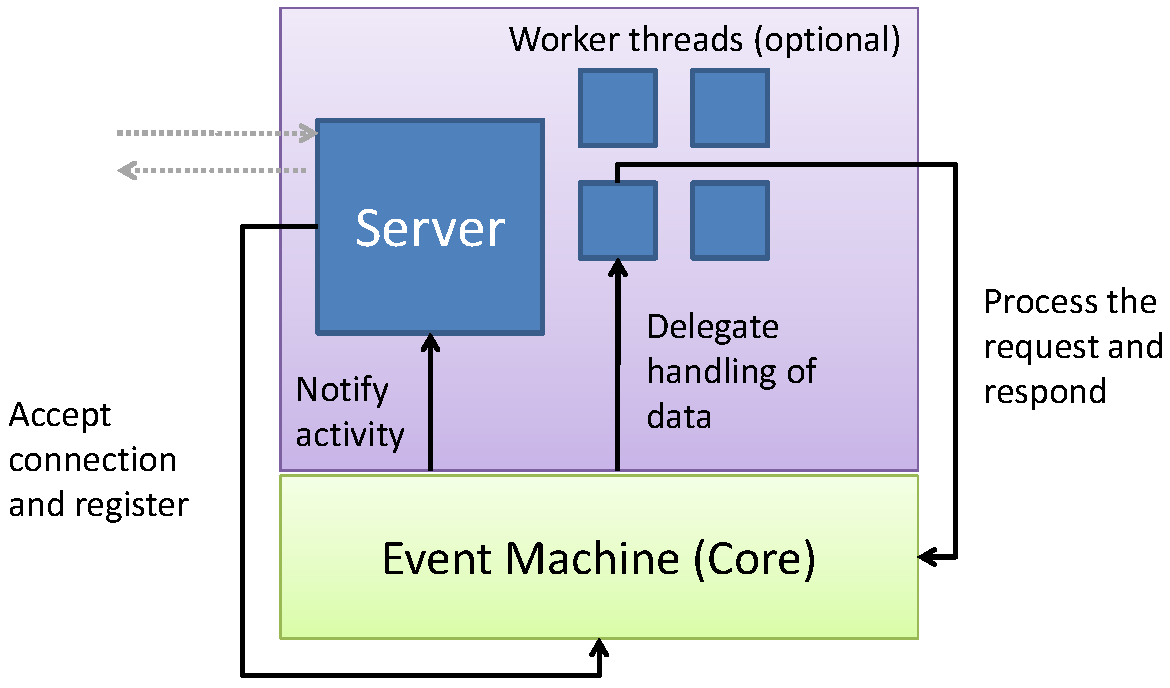
\includegraphics[width=0.75\textwidth]{thin_architecture}
\end{figure}
This setup yields better performance and scalability than Mongrel, especially when serving small requests like, for example, API calls. This is mainly related to the fact that this web server does not launch a new thread for each request, requiring less memory and no context switches~\cite{ruby_webservers}.
 

\subsection{Passenger}
Passenger was also released in 2008 but it had a big difference from the other alternatives since it was not a self-contained web server. Passenger makes use of established web servers like Apache or Nginx by using their reliable web stack. It is mostly written in C++ and used as a module or extension to these generic web servers, adding the needed functionality to support Ruby and handling certain types of requests~\cite{passenger_whatis}.

When the web server starts, having Passenger loaded as a module, it launches a Ruby process that will be responsible for all the other processes handling the Ruby application, called ``worker processes''. Each request is delivered to the firstly created Ruby processes---the master process---which forwards it to one of its workers. These worker processes are single threaded and handle one request at a time~\cite{ruby_webservers}. Passenger's request handling is demonstrated on figure~\ref{fig:passenger_architecture}.
\begin{figure}[h!t]
  \centering
  \caption{Passenger's Request Handling Process}
  \label{fig:passenger_architecture}
    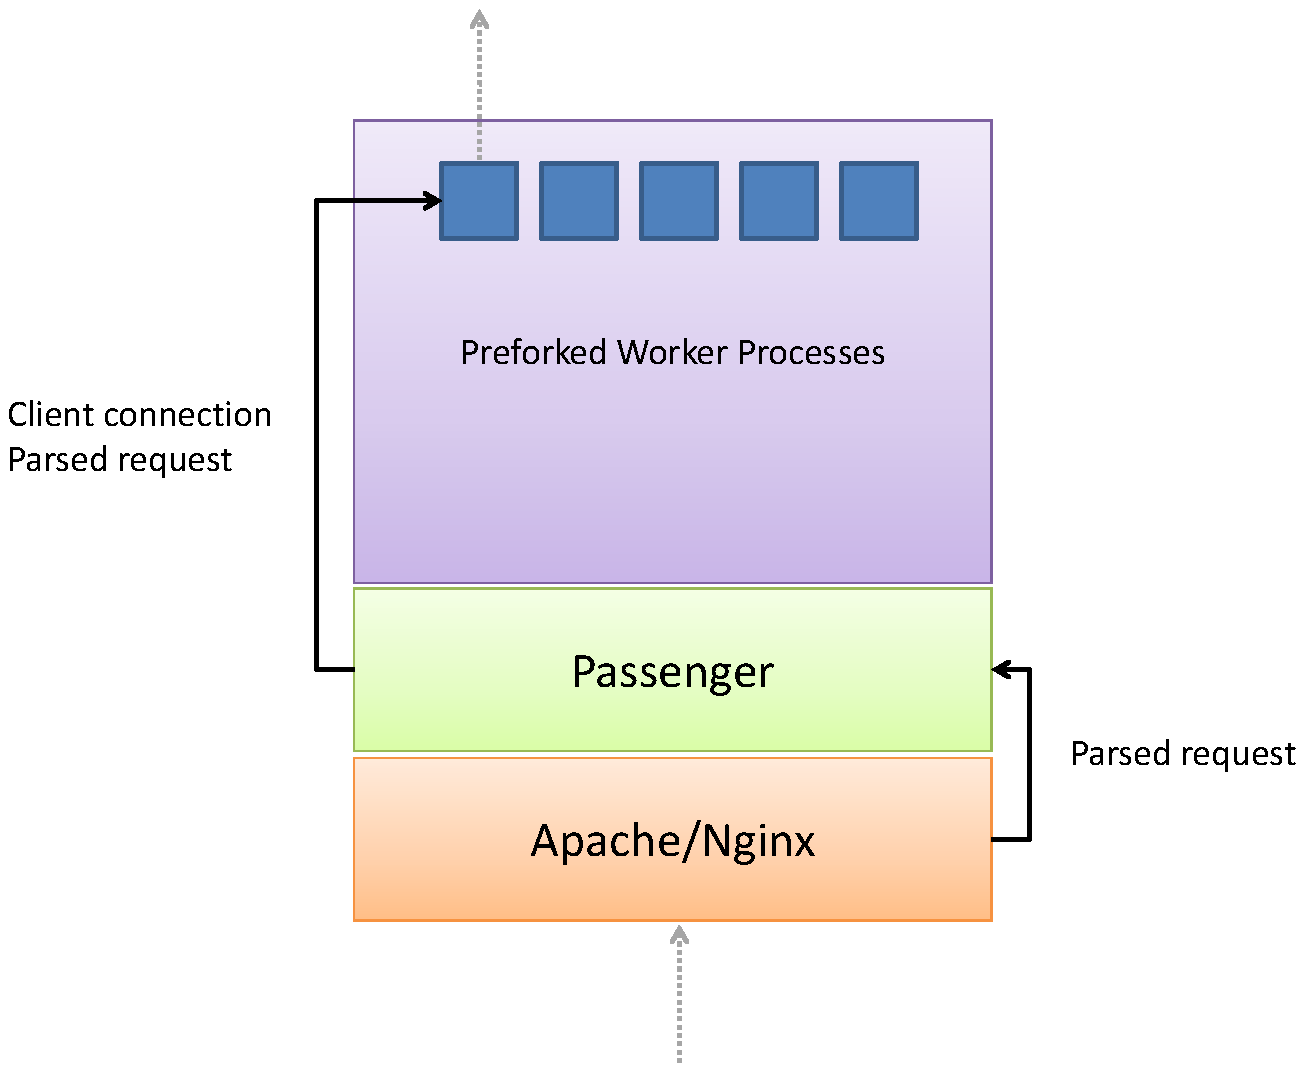
\includegraphics[width=0.75\textwidth]{passenger_architecture}
\end{figure}
It is the first real multi-process server for Ruby, although setups with multiple Mongrel or Thin processes behind a reverse proxy were already being used~\cite{passenger_whatis}. Passenger is a free, open-source product but \textit{Phusion} also provides commercial support.


\subsubsection{Apache}
The Apache HTTP Server is a full-featured and open source web server created by the Apache Software Foundation. It consists on a general purpose web server and provides many useful features such as HTTPS, IPV6 and authentication. Apache natively handles many languages such as PHP and Perl~\cite{apache_features}. It can be extended with modules and this is where Passenger comes in---it will act as \textit{mod\_rails} and extend Apache's functionality to be able to handle Ruby on Rails' applications~\cite{passenger_whatis}.


\subsubsection{Nginx}
Nginx is a general purpose lightweight open source web server with a strong focus on performance~\cite{nginx_features}. It was created by Igor Sysoevy and Passenger can extend its functionality by being installed as a module, similarly to the Apache's procedure~\cite{passenger_whatis}.


\subsection{Unicorn}
Unicorn's first stable version was released in 2009. It is a self-contained web server designed to take advantage of Unix-based kernels and is optimized for fast clients with low latency~\cite{unicorn}. It delegates every task that is better supported by the operating system, Nginx or Rack to themselves, respectively. It uses one master process that spawns and reaps a user-defined number of worker processes without any thread usage. One of its main features is that load balancing is done entirely by the OS kernel, avoiding that requests pile up behind a busy worker. Unicorn is written in Ruby, except for its HTML parser which is based on Mongrel's and, consequently, is written in C. When used in a production environment it should be deployed in conjunction with a reverse proxy capable of fully buffering both the requests and responses between itself and a slow client.
Unicorn's request handling is demonstrated on figure~\ref{fig:unicorn_architecture}.
\begin{figure}[h!t]
  \centering
  \caption{Unicorn's Request Handling Process}
  \label{fig:unicorn_architecture}
    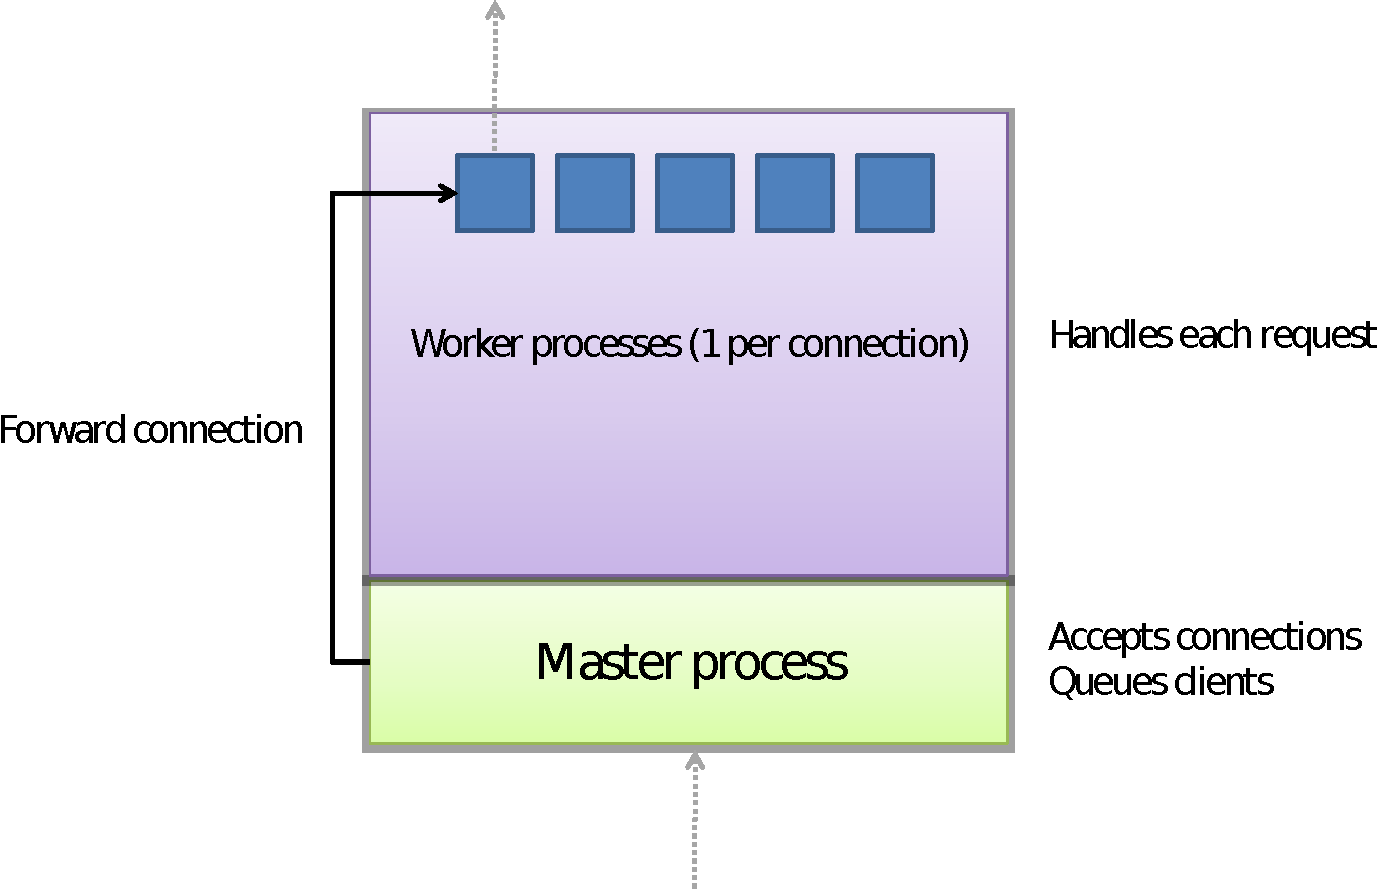
\includegraphics[width=0.75\textwidth]{unicorn_architecture}
\end{figure}
